\begin{frame}[t]{Background}
    
\begin{figure}[h]
    \centering
    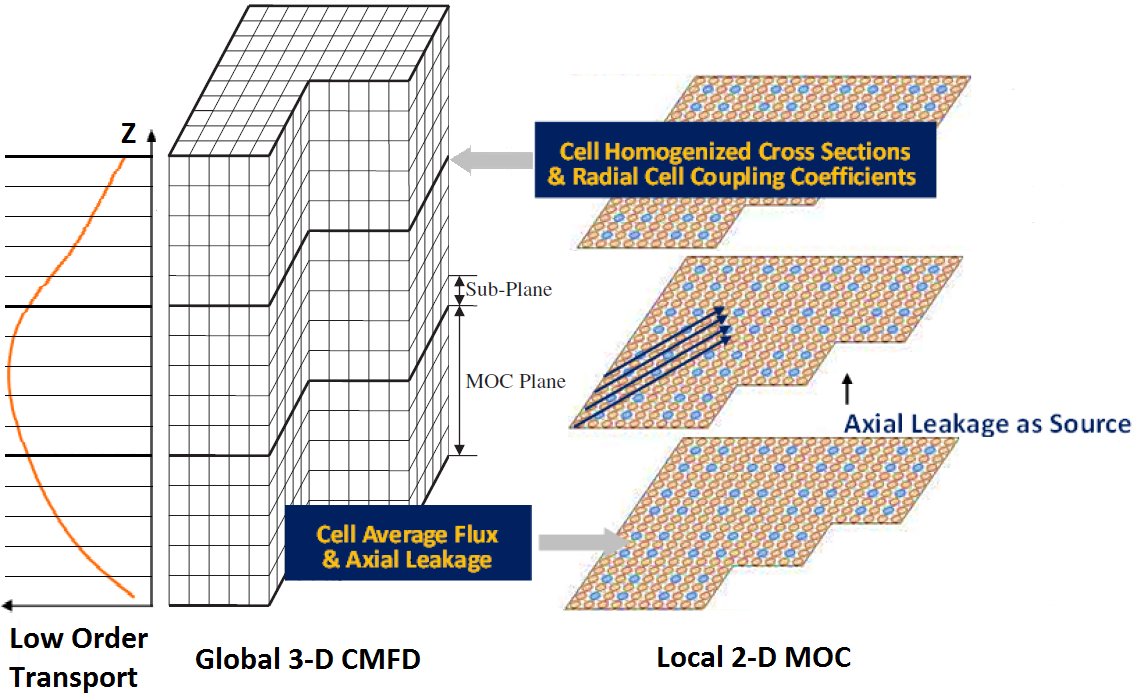
\includegraphics[width=0.8\textwidth]{../figs/2d1d-subplane.png}
    \caption[2D/1D Illustration]{The 2D/1D Method illustrated with the sub-plane scheme for the axial and CMFD calculations}
\end{figure}    
    
\end{frame}

%%%%%%%%%%%%%%%%%%%%%%%%%%%%%%%%%%%%%%%%%%%%%%%%%%%%%%%%%%%%%%%%%%%%%%%%%%%%%%%%%

\begin{frame}[t]{Radial Equations}
    
\begin{subequations}
    \begin{dmath}
        {\Omega_x\frac{\partial \psi_{g}^Z}{\partial x} + \Omega_y\frac{\partial \psi_{g}^Z}{\partial y}} + {\Sigma_{t,g}\left(x,y\right)\psi_{g}^Z\left(x,y,\bm\Omega\right)} = {q_{g}^Z\left(x,y\right)} + {L_{g}^Z\left(x,y,\Omega_z\right)}
    \end{dmath}
    \begin{dmath}
        {q_{g}^Z\left(x,y\right)} = {\frac{1}{4\pi}\sum_{g'=1}^{G}\intop_{4\pi}\Sigma_{s,g'\rightarrow g}^Z\left(x,y,\bm\Omega'\cdot\bm\Omega\right)\psi_{g'}^Z\left(x,y,\bm\Omega'\right)d\Omega'} + {\frac{1}{k_{eff}}\frac{\chi_{g}^Z}{4\pi}\sum_{g'=1}^G\intop_{4\pi} \nu\Sigma_{f,g'}^Z\left(x,y\right)\psi_{g'}^Z\left(x,y,\bm\Omega'\right)d\Omega'} + {\frac{Q_{g}^Z\left(x,y\right)}{4\pi}}
    \end{dmath}
    \begin{align}
    L_{g}^Z\left(x,y,\Omega_z\right) &= \frac{\Omega_z}{\Delta z_k}\left(\psi_{g,z_{k-\frac{1}{2}}} - \psi_{g,z_{k+\frac{1}{2}}}\right) \approx \frac{J_{g,z_{k-\frac{1}{2}}} - J_{g,z_{k+\frac{1}{2}}}}{4\pi\Delta z_k}
    \end{align}
\end{subequations}
    
\end{frame}

%%%%%%%%%%%%%%%%%%%%%%%%%%%%%%%%%%%%%%%%%%%%%%%%%%%%%%%%%%%%%%%%%%%%%%%%%%%%%%%%%

\begin{frame}[t]{Axial Equations}
    
    \begin{subequations}\label{e:2D1DaxialEq}
        \begin{dmath}
            {\Omega_z \frac{\partial \psi_{g}^{XY}}{\partial z}} + {\Sigma_{t,g}^{XY}\left(z\right)\psi_{g}^{XY}\left(z,\bm\Omega\right)} = q_{g}^{XY}\left(z,\Omega_x,\Omega_y\right) + {L_{g}^{XY}\left(z,\Omega_x,\Omega_y\right)}
        \end{dmath}
        \begin{dmath}
            {q_{g}^{XY}\left(z,\Omega_x,\Omega_y\right) = \frac{1}{4\pi}\sum_{g'=1}^G\intop_{4\pi} \Sigma_{s,g'\rightarrow g}^{XY}\left(z,\bm\Omega'\cdot\bm\Omega\right)\psi_{g'}^{XY}\left(z,\bm\Omega'\right)d\Omega'} + {\frac{1}{k_{eff}}\frac{\chi_{g}^{XY}}{4\pi}\sum_{g'=1}^G\intop_{4\pi}\nu\Sigma_{f,g'}^{XY}\left(z\right)\psi_{g'}^{XY}\left(z,\bm\Omega'\right)d\Omega' + \frac{Q_{g}^{XY}\left(z\right)}{4\pi}}
        \end{dmath}
    \end{subequations}
    
\end{frame}

%%%%%%%%%%%%%%%%%%%%%%%%%%%%%%%%%%%%%%%%%%%%%%%%%%%%%%%%%%%%%%%%%%%%%%%%%%%%%%%%%

\begin{frame}[t]{Axial Equations}

\begin{subequations}\label{e:2D1DaxialEq}
    \begin{dmath}
        {\Omega_z \frac{\partial \psi_{g}^{XY}}{\partial z}} + {\Sigma_{t,g}^{XY}\left(z\right)\psi_{g}^{XY}\left(z,\bm\Omega\right)} = q_{g}^{XY}\left(z,\Omega_x,\Omega_y\right) + {L_{g}^{XY}\left(z,\Omega_x,\Omega_y\right)}
    \end{dmath}
    \begin{align}
        L_{g}^{XY}\left(z,\Omega_x,\Omega_y\right) &= {\frac{\Omega_x}{\Delta y_i}\intop_{y_{i-\frac{1}{2}}}^{y_{i+\frac{1}{2}}} \left(\psi_{g,x_{i-\frac{1}{2}}}\left(y\right) - \psi_{g,x_{i+\frac{1}{2}}}\left(y\right) dy\right)} \nonumber\\ 
        &+ {\frac{\Omega_y}{\Delta x_i}\intop_{x_{i-\frac{1}{2}}}^{x_{i+\frac{1}{2}}} \left(\psi_{g,y_{i-\frac{1}{2}}}\left(x\right) - \psi_{g,y_{i+\frac{1}{2}}}\left(x\right) dx\right)} \nonumber\\
        &\approx {\frac{J_{g,x_{i-\frac{1}{2}},y_j} - J_{g,x_{i+\frac{1}{2}},y_j}}{4\pi\Delta x_i}} +
        \frac{J_{g,x_i,y_{j-\frac{1}{2}}} - J_{g,x_i,y_{j+\frac{1}{2}}}}{4\pi\Delta y_j}
    \end{align}
\end{subequations}

\end{frame}

%%%%%%%%%%%%%%%%%%%%%%%%%%%%%%%%%%%%%%%%%%%%%%%%%%%%%%%%%%%%%%%%%%%%%%%%%%%%%%%%%

\begin{frame}[t]{Calculation Flow}

\begin{figure}[h]
    \centering
    \scalebox{0.4}{\begin{tikzpicture}[node distance=2cm]

% Begin
\node (start) [startstop] {Start};
\node (init) [io, right of=start, xshift=2.0cm] {Input, Initialize Solution};

% CMFD
\node (CMFD) [process, below of=init] {CMFD Eigenvalue Calculation};

% Nodal
\node (Nodal) [process, below of=CMFD] {Axial P$_3$ Calculation};

% MOC
\node (MOC) [process, below of=Nodal] {2D MOC Sweeps};

% Finish
\node (convCheck) [decision, below of=MOC, yshift=-1.5cm] {Fission Source, k-eff Converged?};
\node (out) [io, below of=convCheck,yshift=-1.5cm] {Output};
\node (stop) [startstop, right of=out, xshift=2.0cm] {Stop};

% Basic Arrows
\draw [arrow] (start) -- (init);
\draw [arrow] (init) -- (CMFD);
\draw [arrow] (CMFD) -- (Nodal);
\draw [arrow] (Nodal) -- (MOC);
\draw [arrow] (MOC) -- (convCheck);
\draw [arrow] (out) -- (stop);

% Fancy Arrows
\draw [arrow] (convCheck) -- node[anchor=west] {yes} (out);
\draw [arrow] (convCheck) -| node[anchor=north] {no} ([xshift=1.5cm]Nodal.east) |- (CMFD);

\end{tikzpicture}}
    \caption{Calculation flow for 2D/1D scheme}\label{f:2d1d-flowchart}
\end{figure}

\end{frame}

%%%%%%%%%%%%%%%%%%%%%%%%%%%%%%%%%%%%%%%%%%%%%%%%%%%%%%%%%%%%%%%%%%%%%%%%%%%%%%%%%

\begin{frame}[t]{Sub-Plane CMFD}
    
    \begin{figure}[h]
        \centering
        \scalebox{0.4}{\begin{tikzpicture}[node distance=2cm]

% Start
\node (start) [startstop] {Start};

% CMFD
\node (homog) [process, right of=start, xshift=2.0cm] {Homogenize Cross-sections and Flux; Calculate $\tilde{D}$};
\node (iterCheck) [decision, below of=homog, yshift=-1.5cm] {First Iteration?};
\node (firstIter) [process, below of=iterCheck, xshift=-2.5cm, yshift=-1.0cm] {Set $\hat{D}=0$};
\node (laterIter) [process, below of=iterCheck, xshift=2.5cm, yshift=-1.0cm] {Calculate $\hat{D}$};
\node (matrix) [process, below of=firstIter, xshift=2.5cm] {Set up CMFD Matrix};
\node (3DCMFD) [process, below of=matrix] {3D CMFD Calculation};
\node (proj) [process, below of=3DCMFD] {Scale MOC flux with CMFD flux};

% Stop
\node (stop) [startstop, right of=proj, xshift=2.0cm] {Stop};

% Basic Arrows
\draw [arrow] (start) -- (homog);
\draw [arrow] (homog) -- (iterCheck);
\draw [arrow] (matrix) -- (3DCMFD);
\draw [arrow] (3DCMFD) -- (proj);
\draw [arrow] (proj) -- (stop);

% Fancy Arrows
\draw [arrow] (iterCheck) -| node[anchor=south] {yes} (firstIter);
\draw [arrow] (iterCheck) -| node[anchor=south] {no} (laterIter);
\draw [arrow] (firstIter) |- (matrix);
\draw [arrow] (laterIter) |- (matrix);

\end{tikzpicture}}
        \caption{Calculation flow for 3D sub-plane CMFD}\label{f:CMFD-flowchart}
    \end{figure}
    
\end{frame}

%%%%%%%%%%%%%%%%%%%%%%%%%%%%%%%%%%%%%%%%%%%%%%%%%%%%%%%%%%%%%%%%%%%%%%%%%%%%%%%%%

\begin{frame}[t]{1D SP$_3$-NEM}
    
    \begin{figure}[h]
        \centering
        \scalebox{0.6}{\begin{tikzpicture}[node distance=2cm]

% Begin
\node (start) [startstop] {Start};

% Nodal
\node (radialTL) [process, right of=start, xshift=2.5cm] {Calculate radial transverse leakage source};
\node (sp3-0) [process, below of=radialTL] {Solve 0th moment equation};
\node (sp3-2) [process, below of=sp3-0] {Solve 2nd moment equation};
\node (convCheck) [decision, below of=sp3-2, yshift=-1.5cm] {Converged?};

% Stop
\node (stop) [startstop, right of=convCheck, xshift=2.5cm] {Stop};

% Basic Arrows
\draw [arrow] (start) -- (radialTL);
\draw [arrow] (radialTL) -- (sp3-0);
\draw [arrow] (sp3-0) -- (sp3-2);
\draw [arrow] (sp3-2) -- (convCheck);
\draw [arrow] (convCheck) -- node[anchor=north] {yes} (stop);

% Fancy Arrows
\draw [arrow] (convCheck) -| node[anchor=north] {no} ([xshift=-1.5cm]sp3-2.west) |- (sp3-0);

\end{tikzpicture}}
        \caption{Calculation flow for 1D axial calculations in MPACT}\label{f:Axial-flowchart}
    \end{figure}
    
\end{frame}

%%%%%%%%%%%%%%%%%%%%%%%%%%%%%%%%%%%%%%%%%%%%%%%%%%%%%%%%%%%%%%%%%%%%%%%%%%%%%%%%%

\begin{frame}[t]{2D MOC}

\begin{figure}[h]
    \centering
    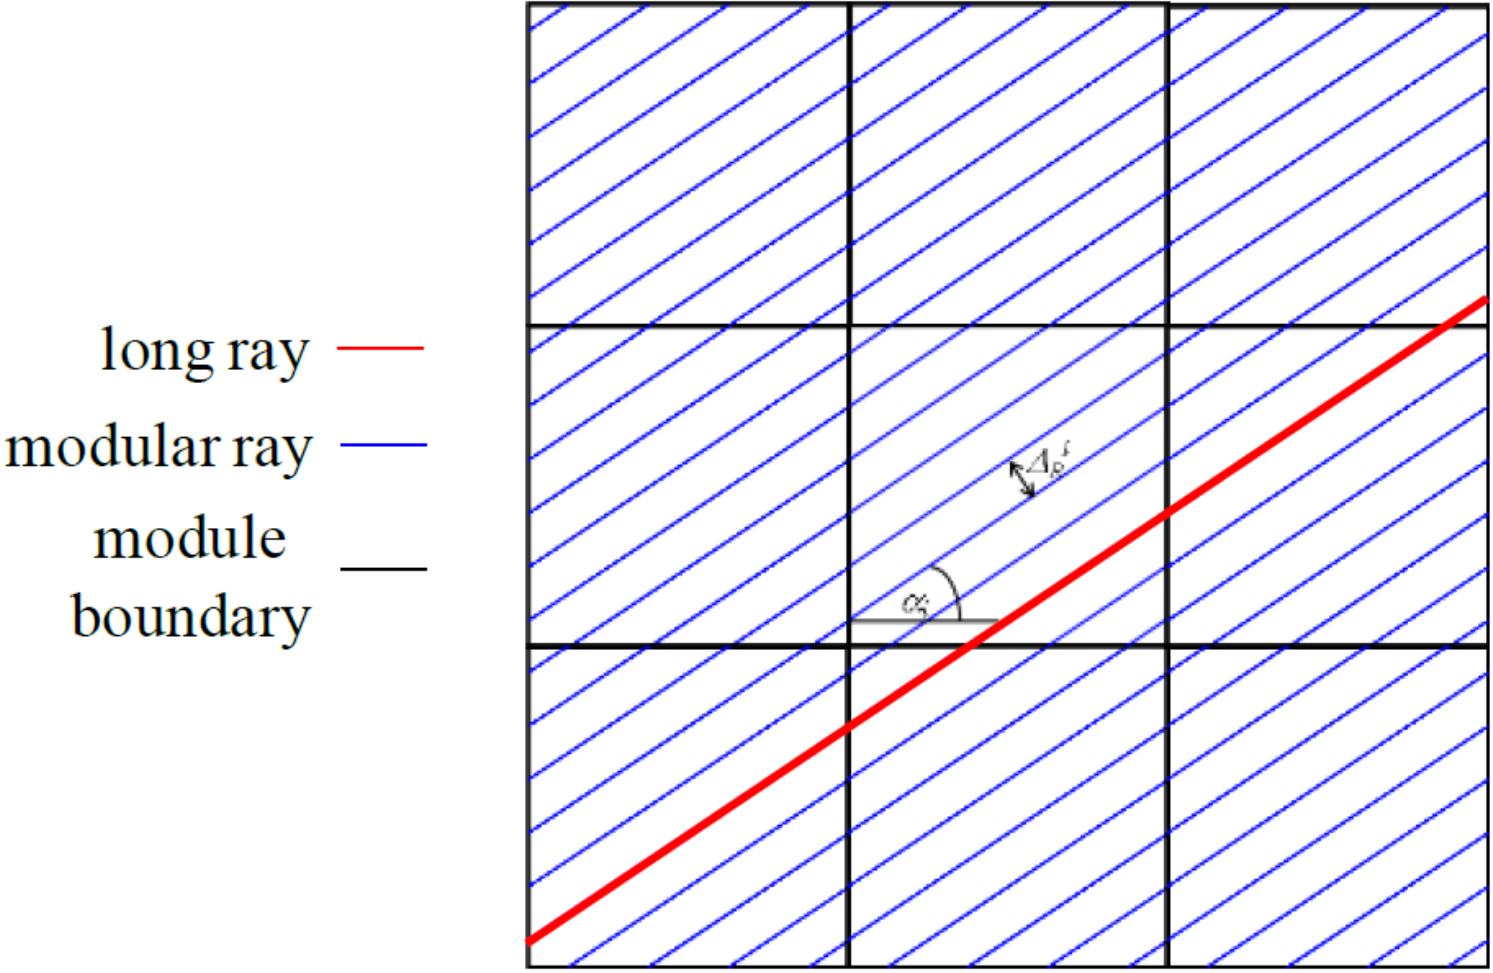
\includegraphics[width=0.5\textwidth]{modular_rays.png}
    \caption[Modular Ray Tracing]{Modular ray tracing depiction \cite{MPACTTheoryManual}}\label{e:ModRays}
\end{figure}

\end{frame} 

%%%%%%%%%%%%%%%%%%%%%%%%%%%%%%%%%%%%%%%%%%%%%%%%%%%%%%%%%%%%%%%%%%%%%%%%%%%%%%%%%

\begin{frame}[t]{2D MOC}

\begin{figure}[h]
    \centering
    \scalebox{0.5}{\begin{tikzpicture}[node distance=2cm]

% Begin
\node (start) [startstop] {Start};
\node (init) [io, right of=start, xshift=2.5cm] {Input N$_{inners}$};

% MOC
\node (begin) [process, below of=init] {Set $n=0$};
\node (source) [process, below of=begin] {Calculate fission and axial transverse leakage sources};
\node (scatSource) [process, below of=source] {Calculate scattering source};
\node (MOC) [process, below of=scatSource] {2D MOC sweep over each energy group};
\node (MOCdone) [decision, below of=MOC, yshift=-1.5cm] {$n = N_{inners}$?};z
\node (stop) [startstop, right of=MOCdone, xshift=2.5cm] {Stop};

% Basic Arrows
\draw [arrow] (start) -- (init);
\draw [arrow] (init) -- (begin);
\draw [arrow] (begin) -- (source);
\draw [arrow] (source) -- (scatSource);
\draw [arrow] (scatSource) -- (MOC);
\draw [arrow] (MOC) -- (MOCdone);

% Fancy Arrows
\draw [arrow] (MOCdone) -| node[anchor=north] {no} ([xshift=-1.5cm]MOC.west) |- (scatSource);
\draw [arrow] (MOCdone) -- node[anchor=north] {yes} (stop);

\end{tikzpicture}}
    \caption{Calculation flow for 2D MOC calculation in MPACT}\label{f:MOC-flowchart}
\end{figure}

\end{frame} 